\documentclass[twocolumn,article]{memoir}
\usepackage{graphicx}
\usepackage{amsmath}
\usepackage{hyperref}
\usepackage{xspace}
\usepackage{courier}
\usepackage{siunitx}

\usepackage[natbib=true,backend=biber,uniquename=init,giveninits=true]{biblatex}

\addbibresource{bibl.bib}
\newcommand\erf{\ensuremath{\mathrm{erf}}\xspace}
\newcommand\erfi{\ensuremath{\mathrm{erfi}}\xspace}
\newcommand\erfc{\ensuremath{\mathrm{erfc}}\xspace}

\newcommand\dx[1]{\,\text{d}#1}

\author{Mark L. Winther}
\title{The Bessel function}

\begin{document}
\twocolumn[
\maketitle

\begin{abstract}
\noindent This project seeks to make a program capable of solving the Bessen function numerically. According to the current list, it is not the project i was supposed to make, but at the time i started doing this project, it was the project i was listed to make. The solution lies close to the library function, and only deviates on a very small numerical scale.
\end{abstract}
]



\subsection*{Introduction}
The purpose of this project is to make a program that is able to solve the Bessel function numerically for the first kind of integer index, via the integral representation. The underlaying purpose is for the author of this project to learn more about coding and solving mathematical problems via numerical methods.

\subsection*{Theory}
\emph{Based on the material from \cite{wiki}.}

Bessel functions are canonical solutions to Bessel's differential equation
\begin{align}
	x^2\frac{d^2y}{dx^2}+x\frac{dy}{dx}+\left(x^2-\alpha^2\right)y=0,
\end{align}
where $\alpha$ is an arbitrary complex number. The most important and applicable solutions are however when $\alpha$ is a real integer. A specific instance of these solutions are defined as Bessel functions of the first kind $J_\alpha(x)$, which are finite at $x=0$ for intiger or positive $\alpha$ but diverge as $x$ approaches zero for negative non-integer $\alpha$. Through series expansion it can be defined as
\begin{align}
	J_\alpha(x) = \sum_{m=0}^\infty \frac{\left(-1\right)^m}{m!\Gamma\left(m+\alpha+1\right)}\left(\frac{x}{2}\right)^{2m+\alpha},
\end{align}
where $\Gamma(k)$ is the gamma function. Limiting it further to only integer values of $\alpha$, defined as $n$, the Bessel function can be represented by the integral
\begin{align}
	J_n(x) = \frac{1}{\pi} \int_0^\pi \cos\left(n\tau-x\sin\tau\right)\dx{\tau},
	\label{eq:Bessel}
\end{align}
which is the representation of the Bessel function that will be solved numerically in this project.

\begin{figure}[ht]
	\centering
	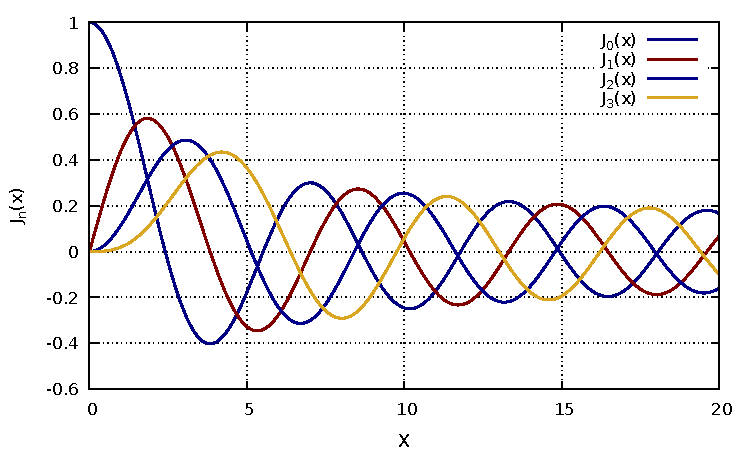
\includegraphics[width=\linewidth]{fig.pdf}
	\caption{The numerically solved Bessel function, for a range of x and n.}
	\label{fig:1}
\end{figure}


\subsection*{Solution}
Firstly, the solution to the problem itself is contained in the program from \texttt{bessel.c}. It is a callable function, that can be called by: \texttt{./bessel n x}, that prints \texttt{x, n, Jn(x), Jg, d} to the standard output, where \texttt{Jn(x)} is the calculated value, \texttt{Jg} is the corresponding value from using the Bessel function from GSL\footnote{https://www.gnu.org/software/gsl/}, and \texttt{d} is the difference between these. The rest of the programs are for extracting plotable data, but use the same way of solving the function. The plot of the functions solved numerically can be seen in Figure \ref{fig:1}, and a plot of its deviation from the GSL function in Figure \ref{fig:2}.

Generally, the program solves the Bessel function by numerical integration, via the use of GSL's numerical integration routine, defined in \texttt{gsl\_integration.h}. When the parameters \texttt{n} and \texttt{x} are given to the program, it sets up the appropriate environment for integration, and solves it via the QAGS algorithm to solve the integral, with both relative and absolute uncertainties set to \num{1e-7}, whereafter the program prints out the result.

The QAGS algorithm solves the the integral by combining adaptive bisection with the Wynn epsilon-algorithm. This allows it to solve integrals with singularities in the integration regoin, by concentrating new subintervals around the singularity. 

\begin{figure}[t]
	\centering
	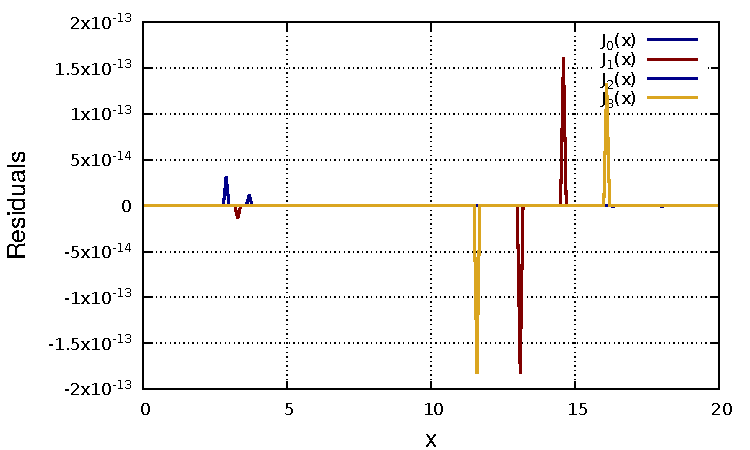
\includegraphics[width=\linewidth]{fig2.pdf}
	\caption{The residuals of the numerically solved Bessel function, for a range of x and n.}
	\label{fig:2}
\end{figure}

\subsection*{Conclusion}

Although the program is simple, and does not do advanced checks of the solutions, it can be seen in Figure \ref{fig:2} that it is quite close to the actual solutions, and shows no systematical errors. Therefore, it is a good approximation to the exact solution.

\printbibliography


\end{document}
